\documentclass[dvips,landscape]{foils}
\usepackage{graphicx,psfrag}
\usepackage{graphics}
\usepackage{amsmath}
\usepackage{amsthm}
\usepackage{amsfonts}
\input defs.tex
\raggedright
\special{! TeXDict begin /landplus90{true}store end }
\renewcommand{\oursection}[1]{
\foilhead[-1.0cm]{#1}
}

\title{Cutoff Phenomenon and Model Reduction}
\author{Tzu-Chen Liang}
\MyLogo{Tzu-Chen Liang, Stanford University}
\date{\today}
\newtheorem{definition}{Definition}
\newtheorem{example}{Example}

\begin{document}
%\setlength{\parskip}{0cm}
\maketitle
%%%%%%%%%%%%%%%%%%%%%%%%%%%%%%%%%%%%%%%%%%%%%%%%%%%%%%%%%%%%%%%%%%%%%%%%%%
%\newpage
%\oursection{Outline}
%\BIT \itemsep -1pt
%\item Motivation
%\item Cutoff Phenomenon
%\item Conclusion
%\EIT
%\vfill
%%%%%%%%%%%%%%%%%%%%%%%%%%%%%%%%%%%%%%%%%%%%%%%%%%%%%%%%%%%%%%%%%%%%%%%%%
\oursection{Motivation}
\begin{itemize}
\item Optimization
 \begin{eqnarray*}
  \begin{array}{cl}
   \textbf{maximize}  &  \text{mixing rate}\\
   \textbf{subject to}&  \text{material constraints, stoke's equation, etc.}
  \end{array}
 \end{eqnarray*}
\item rumor: the second largest eigenvalue of a Markov matrix decides its mixing rate.
\item wouldn't it be good if we model the mixing channel as a Markov chain? 
\end{itemize}
%%%%%%%%%%%%%%%%%%%%%%%%%%%%%%%%%%%%%%%%%%%%%%%%%%%%%%%%%%%%%%%%%%%%%%%%%
\newpage

\includegraphics[width=1\textwidth,trim=1cm 1cm 0cm 11cm]{Standardmapexample}

\textbf{Standard Map}
  \begin{eqnarray*}
               x_1' &\leftarrow&  x_1+x_2 +\epsilon \sin{2 \pi x_1} (\mbox{ mod } 1)\\
               x_2' &\leftarrow&  x_2 +\epsilon \sin{2 \pi x_1}     (\mbox{ mod } 1)
  \end{eqnarray*}


%%%%%%%%%%%%%%%%%%%%%%%%%%%%%%%%%%%%%%%%%%%%%%%%%%%%%%%%%%%%%%%%%%%%%%%%%
\newpage
\centerline{
\begin{tabular}{rl}%\setlength{\tabcolsep}{-30mm}
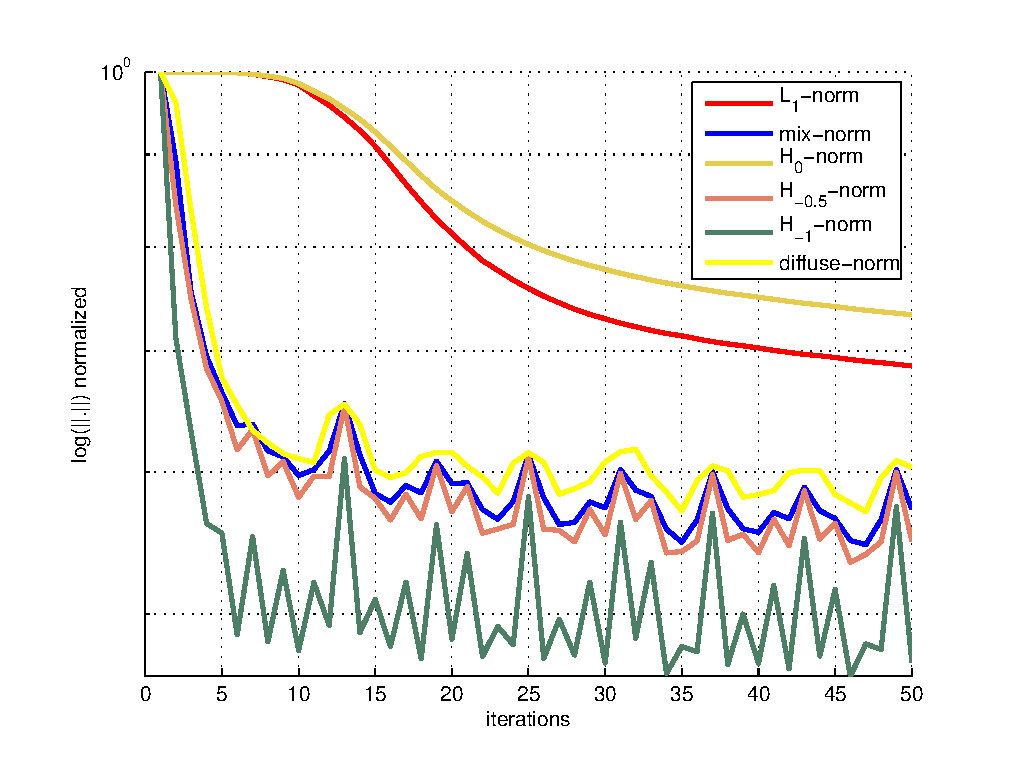
\includegraphics[width=0.53\textwidth,trim=1cm 1cm 0cm 0cm]{lognormplot}&
\includegraphics[width=0.53\textwidth,trim=1cm 1cm 0cm 0cm]{normcompare}
\end{tabular}
}
\begin{itemize}
\item norms are the measures of how well the colors mix
\item $\|f\|_{*} =\hat{f}^T \Lambda_{*} \hat{f} $, where $\hat{f}= \text{DFT}(f)$, $\Lambda_*$ is a diagonal matrix. 
\end{itemize}
%%%%%%%%%%%%%%%%%%%%%%%%%%%%%%%%%%%%%%%%%%%%%%%%%%%%%%%%%%%%%%%%%%%%%%%%%
\newpage
\oursection{Markov Chain}
\begin{itemize}
 \item Finite states, discrete time
 \item Markov property
 \item $X$ denotes the actual state, and $x$ is the distribution, $x_i = \textbf{Prob}\left( X=i\right)$
 \item \textbf{State transition matrix } $P$, $P_{ij} = \textbf{Prob}\left( X^{k+1}=j| X^k=i \right)$ 
 \item $x^{k+1} = P^T x^k$, for $k = 0,1,2,...$
 \item $P^T\pi= \pi$, $P\mathbf{1}=\mathbf{1}$. $\pi$ is the \textbf{invariant distribution}
\end{itemize}
%%%%%%%%%%%%%%%%%%%%%%%%%%%%%%%%%%%%%%%%%%%%%%%%%%%%%%%%%%%%%%%%%%%%%%%%%
\newpage
\begin{example} A Computer
%\centerline{
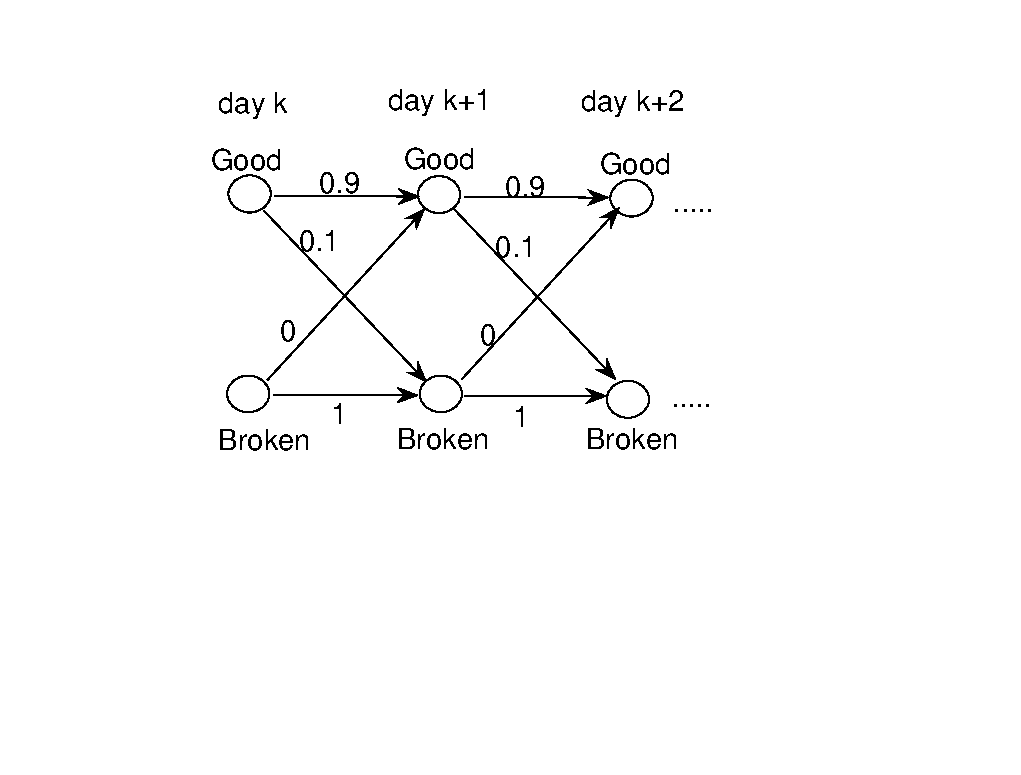
\includegraphics[width=1\textwidth,trim=-3cm 4cm 1cm 0cm]{Markovchainexample}
%}
\begin{eqnarray*}
 P = \left[\begin{array}{c c}
      0.9&0.1\\
      0  & 1 
     \end{array}\right], \mbox{  } 
 \pi = \left[\begin{array}{c}
       0\\
       1 
     \end{array}\right]
\end{eqnarray*}
\end{example}

%%%%%%%%%%%%%%%%%%%%%%%%%%%%%%%%%%%%%%%%%%%%%%%%%%%%%%%%%%%%%%%%%%%%%%%%%
\oursection{Cutoff Phenomenon}

\begin{example} \textbf{Random walk on an $n$-dimensional hypercube}
a particle starts at $\mathbf{0}$ and moves to one of its nearest neighbors (or stay fixed) with equal probability at each step.

\includegraphics[width=0.45\textwidth,trim=1cm 1cm 0cm 0cm]{cutoffexample}
\parbox[b]{12cm}{
  Total Variation Distance
  \begin{eqnarray*}
   \|x - \pi\| &=& \frac{1}{2}\sum_{i=1}^n |x_i-\pi_i |\\
               &=& \frac{1}{2}\sum_{i=1}^n |f_i-1|\pi_i
  \end{eqnarray*}
  where $f_i = x_i/\pi_i$. $f$ is the density of $x$ with respect to $\pi$.
   }

\end{example} 




%%%%%%%%%%%%%%%%%%%%%%%%%%%%%%%%%%%%%%%%%%%%%%%%%%%%%%%%%%%%%%%%%%%%%%%%%
\newpage
Assume that, to any finite set $\Omega$ and any
pair of probability measures $\mu$, $\nu$ on $\Omega$ is associated
a real number $D(\mu,\nu)$ such that $D(\mu,\nu)\in [0,1]$,

\begin{eqnarray}
\max_{\Omega,\mu,\nu} D(\mu,\nu) = 1
\end{eqnarray}
and $D(\mu,\nu)=0$ if and only if $\mu=\nu$. Consider a sequence of
(finite) probability spaces $(\Omega_n,\nu_n)$, $n=1,2,...$, each
equipped with a sequence of probability measure $\mu^k_n$,
$l=0,1,...$, such that
\begin{eqnarray}
\lim_{k \rightarrow \infty} D(\mu^k_n,\nu_n)=0
\end{eqnarray}
%%%%%%%%%%%%%%%%%%%%%%%%%%%%%%%%%%%%%%%%%%%%%%%%%%%%%%%%%%%%%%%%%%%%%%%%%
\newpage
\begin{definition}
\label{cutoffdefition}
(Diaconis) A family $(\Omega_n,\nu_n, (\mu^k_n)_{k=0,1,...})_{n=1,2,...}$
presents a D-cut-off if there exists a sequence $(t_n)$ of positive
reals such that, for any $\epsilon \in(0,1)$,
\begin{enumerate} \setlength{\parskip}{0pt}  \setlength{\itemsep}{-0pt} \setlength{\topsep}{0pt} %\setlength{\parsep}{70pt}% 
  \item $\lim_{k \rightarrow \infty}D(\mu^{k_n}_n,\nu_n) = 0 \mbox{ if }
  k_n>(1+\epsilon)t_n$
  \item $\lim_{k \rightarrow \infty}D(\mu^{k_n}_n,\nu_n) = 1 \mbox{ if }
  k_n<(1-\epsilon)t_n $
\end{enumerate}
\end{definition}
\centerline{
\begin{tabular}{rl}%\setlength{\tabcolsep}{-30mm}
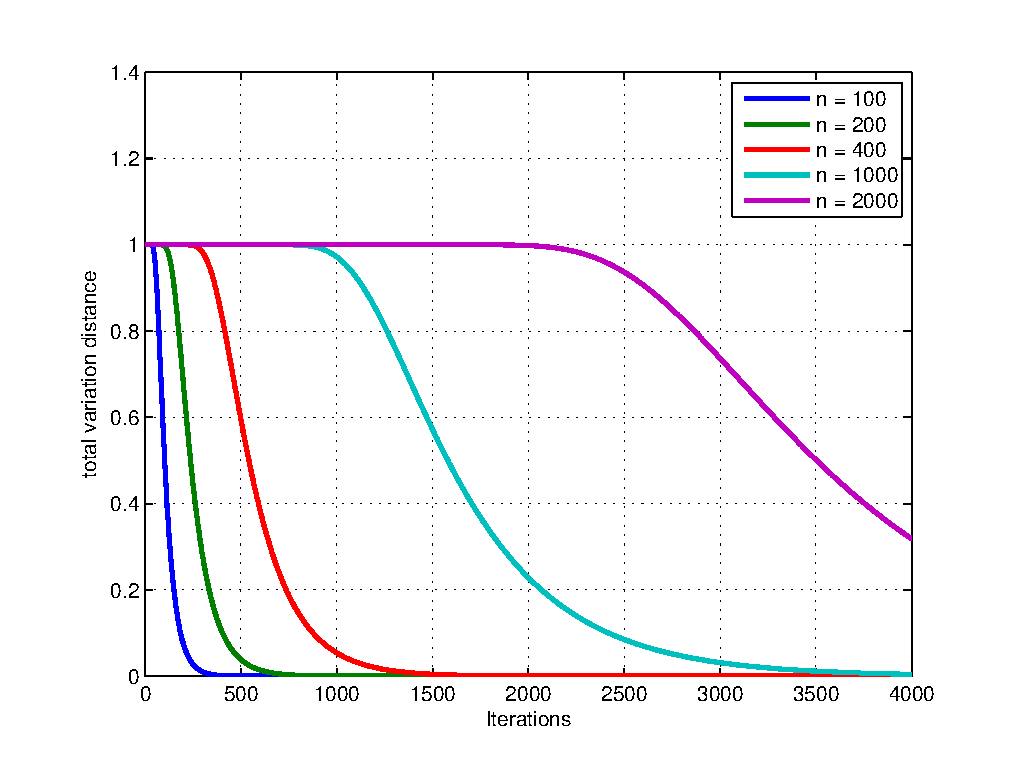
\includegraphics[width=0.43\textwidth,trim=1cm 1cm 0cm 0cm]{rdwalk}&
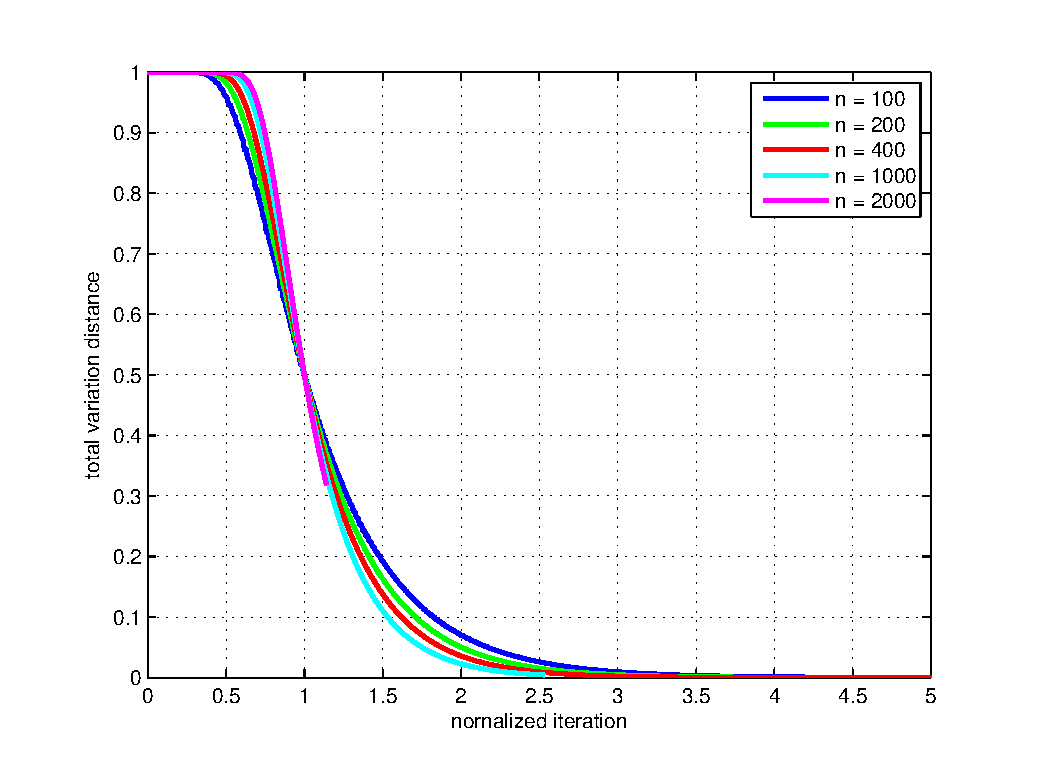
\includegraphics[width=0.43\textwidth,trim=1cm 1cm 0cm 0cm]{rdwalkn}
\end{tabular}
}

%%%%%%%%%%%%%%%%%%%%%%%%%%%%%%%%%%%%%%%%%%%%%%%%%%%%%%%%%%%%%%%%%%%%%%%%%
\newpage
\begin{tabular}{rl}
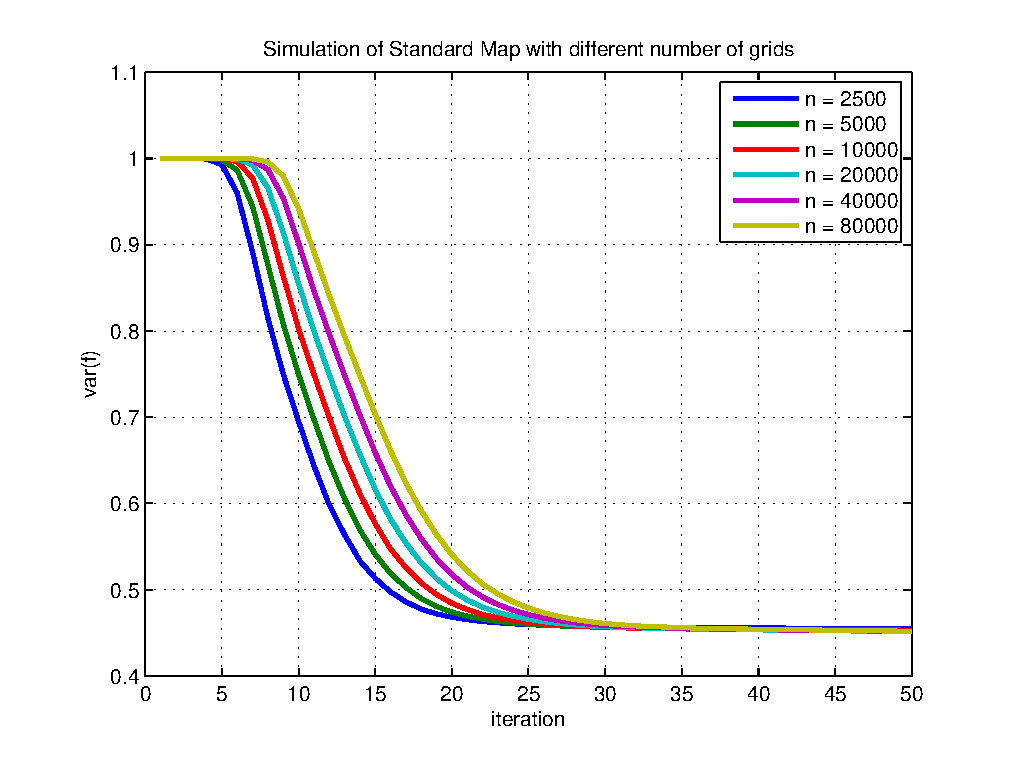
\includegraphics[width=0.50\textwidth,trim=1cm 1cm 0cm 0cm]{standardmapcutoff}&
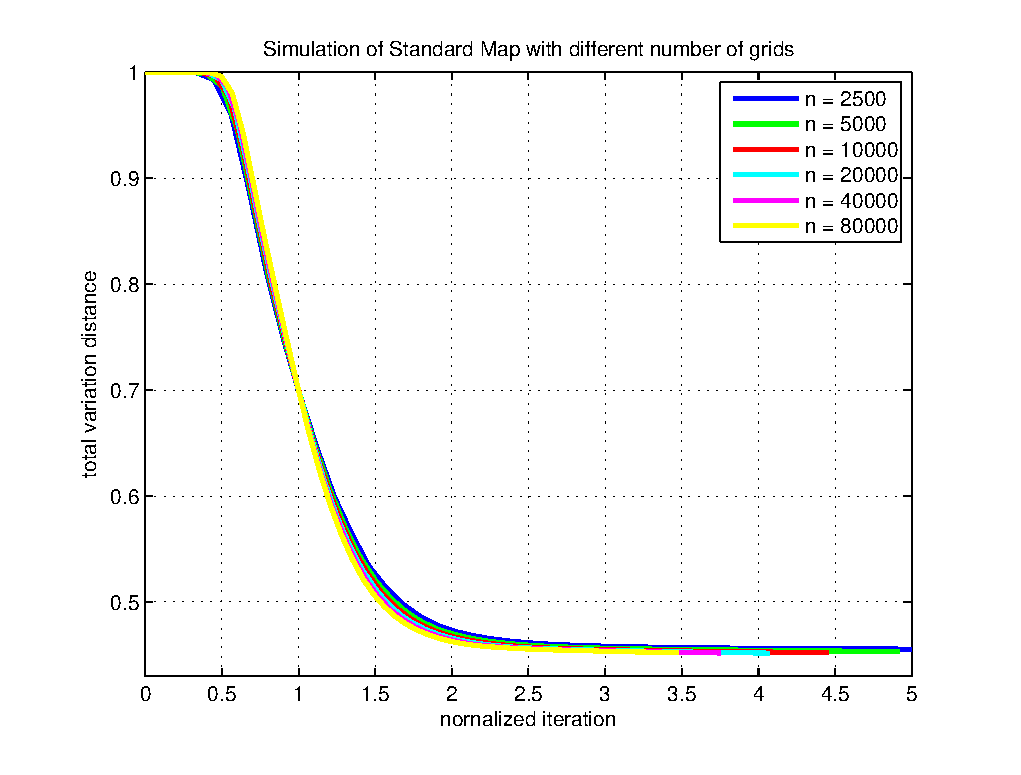
\includegraphics[width=0.50\textwidth,trim=1cm 1cm 0cm 0cm]{standardmapcutoffn}
\end{tabular}
\centerline{
\begin{tabular}{rl}
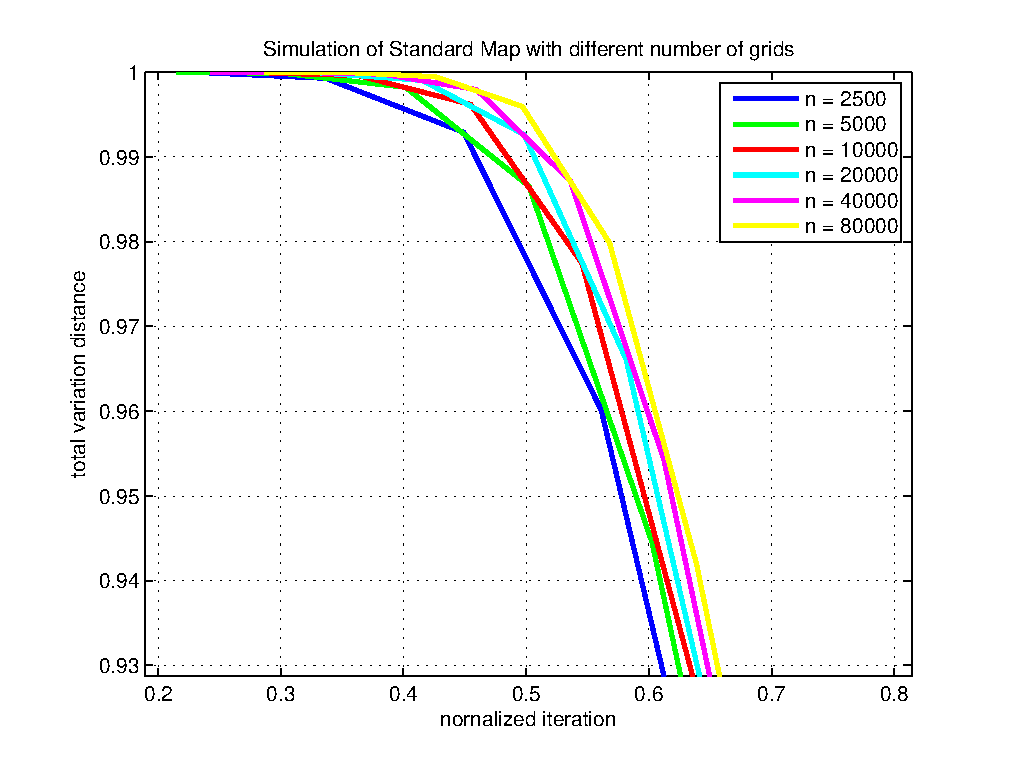
\includegraphics[width=0.28\textwidth,trim=1cm 1cm 0cm 0cm]{standardmapcutoffmacro}
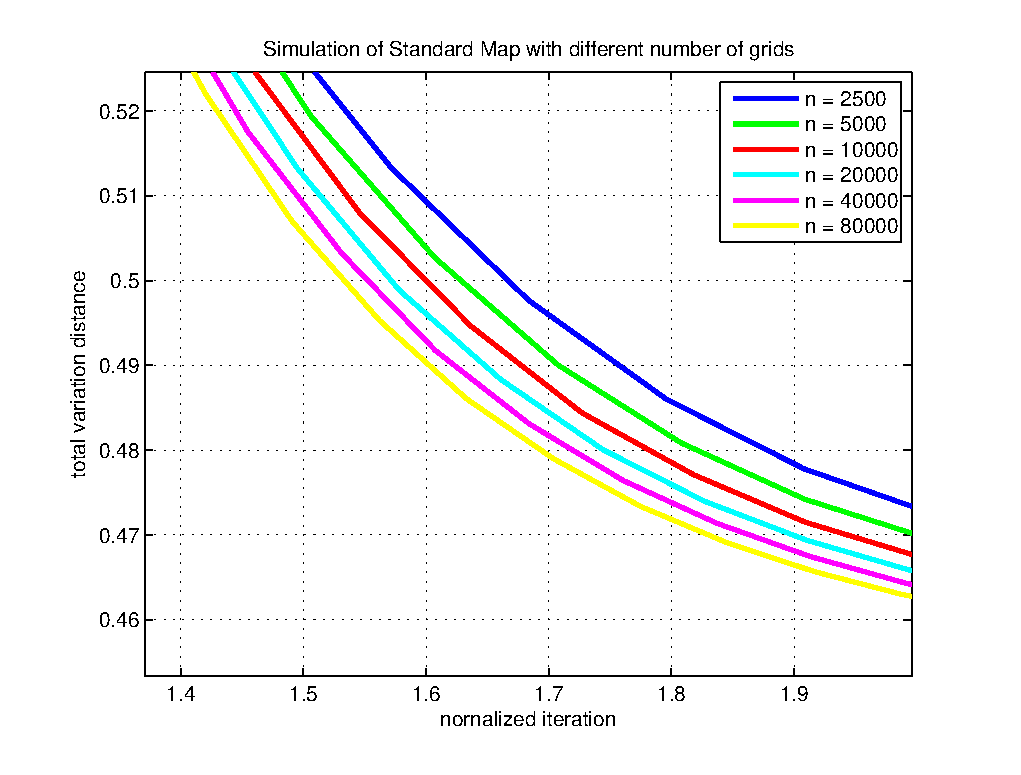
\includegraphics[width=0.28\textwidth,trim=1cm 1cm 0cm 0cm]{standardmapcutoffmacro2}
\end{tabular}
}

%%%%%%%%%%%%%%%%%%%%%%%%%%%%%%%%%%%%%%%%%%%%%%%%%%%%%%%%%%%%%%%%%%%%%%%%%
\newpage
\oursection{The Tool: Model Reduction}
\begin{itemize}
\item Consider a finite state space $X =\mathbb{Z}_n$, and a finite observation space $Y=\mathbb{Z}_m$. $n>m$
\begin{eqnarray*}
   P_{ij}&=&\textbf{Prob}\left( X^{k+1}=j| X^k=i \right)\\
   B_{ij}&=&\textbf{Prob}\left( Y^k=j| X^k=i \right)
\end{eqnarray*}  
\item the "best" model $\bar{P} \in \mathbb{R}^{m \times m}$ of $P \in \mathbb{R}^{n \times n}$ is
\begin{eqnarray*}
  \bar{P} = \Psi_X P \Psi_Y
\end{eqnarray*} 
where $\Psi_X \in \mathbb{R}^{m \times n}$ is fat, and $\Psi_Y \in \mathbb{R}^{n \times m}$ is skinny. They are functions of $B$ and $\pi$
%\item $P$ can be infinite dimensional.
\end{itemize}
%%%%%%%%%%%%%%%%%%%%%%%%%%%%%%%%%%%%%%%%%%%%%%%%%%%%%%%%%%%%%%%%%%%%%%%%%
\newpage
\begin{example} Computer again
\centerline{
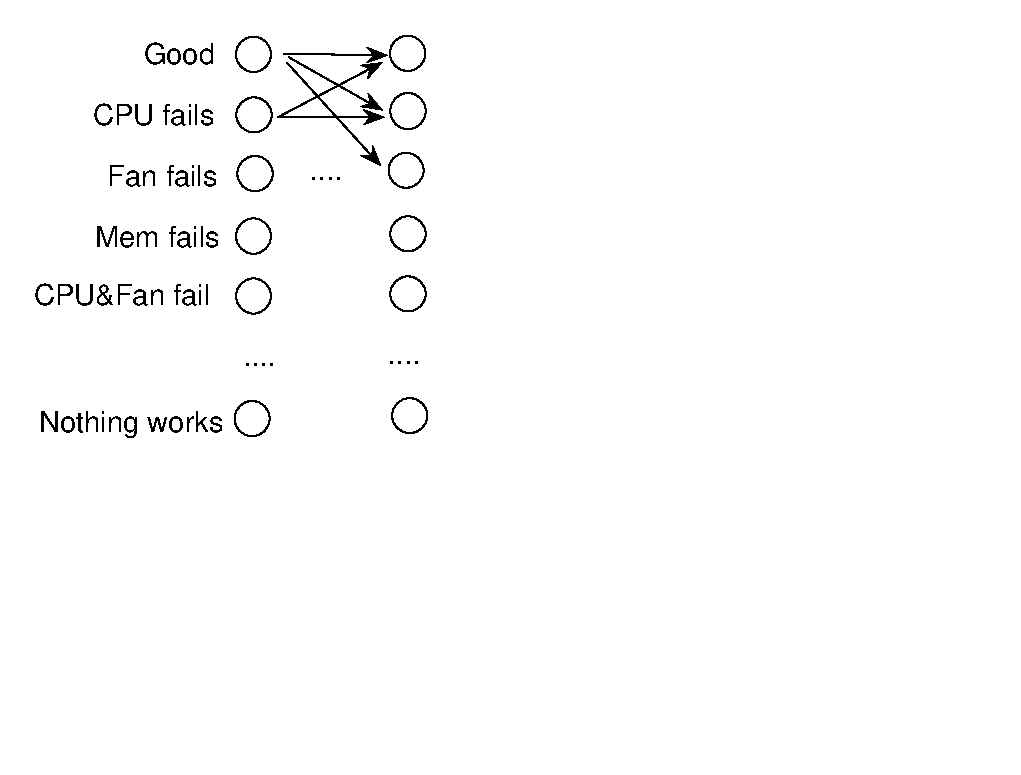
\includegraphics[width=0.5\textwidth,trim=0cm 5cm 7cm 0cm]{Markovchainexample2}
}
\end{example}
\begin{itemize}
\item finite observation: turn on the power, it works or not.
\end{itemize}
%%%%%%%%%%%%%%%%%%%%%%%%%%%%%%%%%%%%%%%%%%%%%%%%%%%%%%%%%%%%%%%%%%%%%%%%%
\newpage
\begin{example} Mixing Channel: What do we lose?
\centerline{
\includegraphics[width=0.65\textwidth]{mixingprocess}
}
\end{example}
%%%%%%%%%%%%%%%%%%%%%%%%%%%%%%%%%%%%%%%%%%%%%%%%%%%%%%%%%%%%%%%%%%%%%%%%%
%\newpage
%\centerline{
%\begin{tabular}{rl}%\setlength{\tabcolsep}{-30mm}
%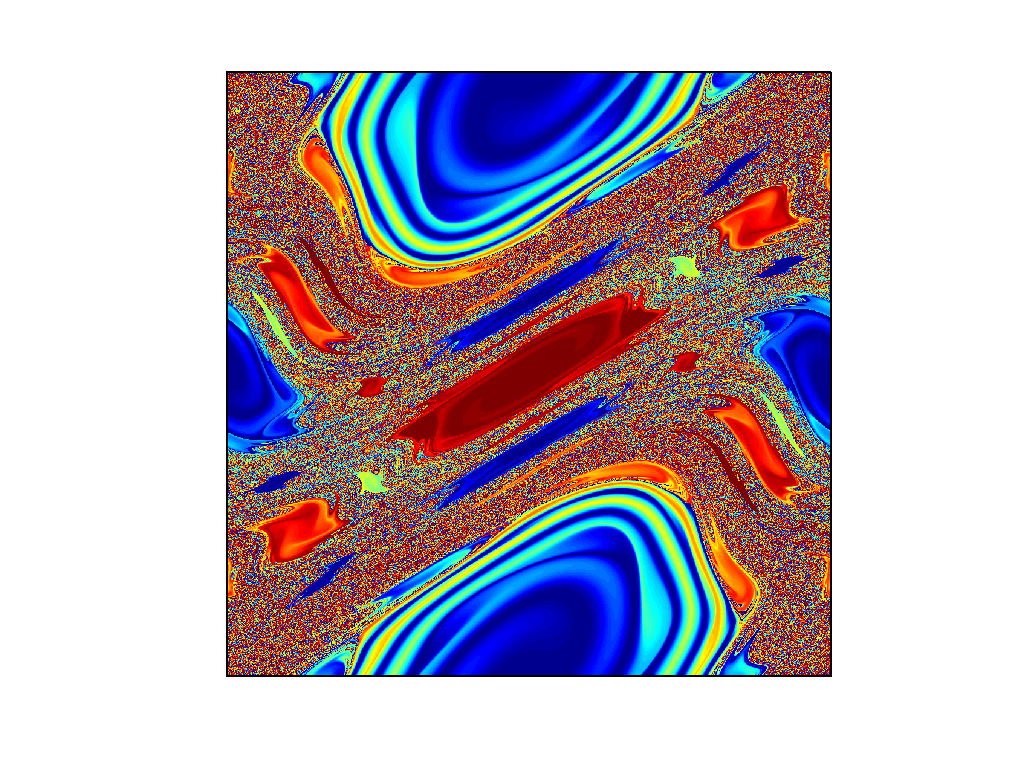
\includegraphics[width=0.55\textwidth,trim=1cm 1cm 0cm 0cm]{standardmapsimuexact}&
%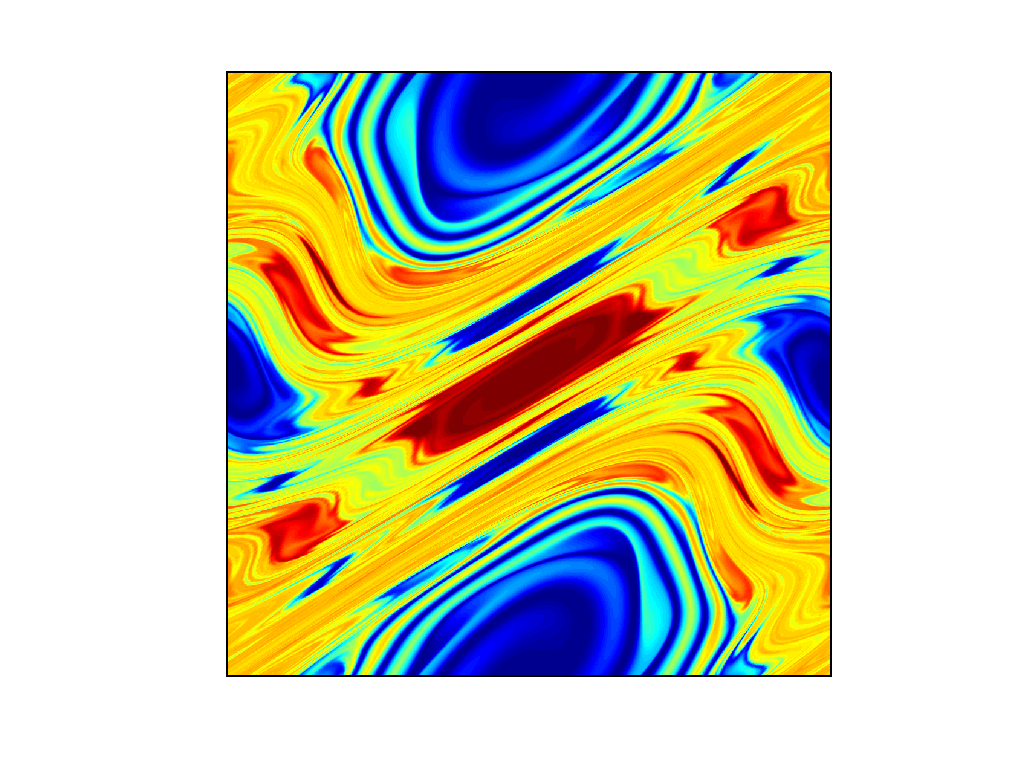
\includegraphics[width=0.55\textwidth,trim=1cm 1cm 0cm 0cm]{standardmapsimumarkov}
%\end{tabular}
%}

%%%%%%%%%%%%%%%%%%%%%%%%%%%%%%%%%%%%%%%%%%%%%%%%%%%%%%%%%%%%%%%%%%%%%%%%%
\newpage
\begin{itemize}
\item Question: when is the reduction exact? i.e.,
      \begin{eqnarray*}
         y^k = B^T x^k, \mbox{for } k=0,1,2,...
      \end{eqnarray*}
\item Answer: 
      \begin{eqnarray*}
      (\Psi_X^T\Psi_Y^T-I)(P^T)^k x^0 =0 \mbox{  , for }k=0,1,...
      \end{eqnarray*}
\item We need to either choose $B$ cleverly or begin the simulation with some very special $x^0$. 
\item This equation says nothing about how to do that. 
\end{itemize}
%%%%%%%%%%%%%%%%%%%%%%%%%%%%%%%%%%%%%%%%%%%%%%%%%%%%%%%%%%%%%%%%%%%%%%%%%
\newpage
\oursection{Model Reduction of Random Walk problem}
\begin{eqnarray*}
B_{ij} = \left\{ \begin{array}{cl}
                 1,&\mbox{ if } i_{th} \mbox{ corner has 1-norm distance } j \mbox{ to the origin}\\
                 0,&\mbox{ otherwise}
                 \end{array} \right.
\end{eqnarray*}
\begin{itemize}
\item Example: on a 3-D cube $(000), (010), (001) \rightarrow 0,1,1,$ respectively. 
\item Reduce the system from $X \in \{1,2,...,2^n\}$ to $Y \in \{0,1,2,..,n\}$. Significant! 
\item The reduced system is called "Ehrenfests' Urn" prbolem.
\end{itemize}
%%%%%%%%%%%%%%%%%%%%%%%%%%%%%%%%%%%%%%%%%%%%%%%%%%%%%%%%%%%%%%%%%%%%%%%%%
\newpage 
\oursection{Ehrenfests' Urn}
\begin{itemize}
\item two urns and $d$ balls. To start, all the balls are in urn $2$. Each time, a ball is randomly chosen and moved to the other urn. 
\item the state of the Markov chain is the number of balls in urn $1$.
\item $\pi_j = {d \choose j}/2^d$
\item The amazing fact: the reduction is exact.
\end{itemize}

%%%%%%%%%%%%%%%%%%%%%%%%%%%%%%%%%%%%%%%%%%%%%%%%%%%%%%%%%%%%%%%%%%%%%%%%%
\newpage
\oursection{Conclusion}
\begin{itemize}
\item Can we find a systematic way to choose $B$ according to $x^0$?
\item If so, can we apply this result to Standard Map?
\item We have a sequence of Markov chain which converges to the true Standard map. Then, what does the sequence of random walk Markov chiain converge to?
\end{itemize}



%%%%%%%%%%%%%%%%%%%%%%%%%%%%%%%%%%%%%%%%%%%%%%%%%%%%%%%%%%%%%%%%%%%%%%%%%
%%%%%%%%%%%%%%%%%%%%%%%%%%%%%%%%%%%%%%%%%%%%%%%%%%%%%%%%%%%%%%%%%%%%%%%%%
%\newpage
\oursection{Example: Riffle Shuffle Problem}
\begin{itemize}
\item The most common method of mixing cards
\item A deck of $n$ cards (often $n=52$) is cut into two parts and the parts are riffled together
\item The basic model of this procedure was introduced by Gilbert and Shannon(1955)
\item Many open questions, and tons of related research fields 
\item The most famous example of cutoff phenomenon
\end{itemize}
%%%%%%%%%%%%%%%%%%%%%%%%%%%%%%%%%%%%%%%%%%%%%%%%%%%%%%%%%%%%%%%%%%%%%%%%%
\newpage
\oursection{GSR Model of Riffle Shuffle}
\begin{itemize}
\item the deck is cut into two piles according to the binomial distribution so the chance that pile one has $j$ cards is ${n \choose j}/2^n$
\item Then, sequentially drop cards from the bottoms of the two piles according to the following rule: if at some stage pile one has $A$ cards and pile two has $B$ cards, drop the next card from pile one with probability $A/(A+B)$
\item This is continued until the two piles are exhausted and then the piles are pushed together.
\end{itemize}
%%%%%%%%%%%%%%%%%%%%%%%%%%%%%%%%%%%%%%%%%%%%%%%%%%%%%%%%%%%%%%%%%%%%%%%%%
\newpage
\oursection{GSR Model of Riffle Shuffle}
\begin{itemize}
\item A Markov chain with $n!$ states (permutations)
\item Question: How many shuffles are necessary and suffice to approximately randomize $52$ cards?
\end{itemize}
\centerline{
\includegraphics[width=0.50\textwidth,trim=1cm 1cm 0cm 0cm]{riffleshuffle}
}
%%%%%%%%%%%%%%%%%%%%%%%%%%%%%%%%%%%%%%%%%%%%%%%%%%%%%%%%%%%%%%%%%%%%%%%%%
%\newpage
%\oursection{The Analysis of GSR Model}
%\begin{itemize}
%\item aa
%\end{itemize}
%%%%%%%%%%%%%%%%%%%%%%%%%%%%%%%%%%%%%%%%%%%%%%%%%%%%%%%%%%%%%%%%%%%%%%%%%
\end{document}


















